\chapter{Hypervisor-based invariance-enforcing framework} \label{hellorootkitty}

\epigraph{2in}{Prediction is very difficult, especially if it's about the future.}{Niels Bohr}{}


Operating systems consist of trusted code that executes directly on top of a host's hardware. This code usually provides several functionalities such as abstraction, essential to develop programs that use the system functions offered by the operating system; arbitration, to allocate resources to more than one concurrently running program in a collision-free fashion and isolation to prevent one program from addressing the memory space of another \cite{stallings}.

Due to their prominent position, operating systems become a common target of attackers who regularly try to circumvent their protection mechanisms and modify them to their advantage. In the past, a malicious program that allowed a user to elevate his access and become a system administrator, or \texttt{root}, was called a \texttt{rootkit}. Today the meaning of rootkits has changed and is used to describe software that hides the attacker's presence from the legitimate system's administrator. 
%A trivial classification of rootkits is based on their main target. Thus, user-mode rootkits target applications in userland and achieve stealth by hiding resources from the operating system arbitration APIs. These types of rootkits are portable and normally characterized by a high attack success rate\cite{usermoderootkit}. Their damage impact is limited by how critical the target application is, but it is often localized by the operating system isolation functionality. 
Kernel-mode rootkits target the core of an operating system. It goes without saying that they are the hardest to detect and remove. Such rootkits appear very often in the form of device drivers (Windows platform) or Loadable Kernel Module (Linux kernel). 
In other cases, a kernel-mode rootkit may be introduced by a software bug in the kernel and  triggered by a malicious or a benign but-exploitable process.
Regardless of the way the rootkit is introduced, the result is malicious code running with operating system privileges which can add and execute additional code or modify existent kernel code. The activities resulting from a successful attack can range from spamming and key-logging to stealing private user-data and disabling security software running on the host.
In the past, rootkits have also been used to turn their targets into nodes of a botnet as with Storm Worm~\cite{1387718} or to perform massive bank frauds ~\cite{mcaffee}.
An even more subtle type of rootkits does not introduce new code at all, but rather makes use of existing fragments of operating system code - that will be considered trusted by any active monitor - to fabricate their malicious functionality. The execution of these fragments in a specific order, chosen by the attacker has give birth to an entirely new way of compromising the kernel called \texttt{return-oriented rookits} \cite{Hund2009}. 

Generally speaking, changing the control flow of the operating system kernel involves either changing the content of specific kernel objects such as existing fragments of code with new code or overwriting kernel function pointers.
Several approaches that mitigate rootkits have been developed by security researchers who consider modified kernel-data structures an evidence of attack. Unfortunately, many of these approaches are affected by substantial overhead~\cite{livewire,5} or miss a fundamental security requirement such as isolation\cite{hookscout}. 
Isolation is needed to prevent a countermeasure in the target system from being disabled or crippled by a potential attack. When malicious code is running at the same privilege level as the operating system kernel, no isolation mechanism is in place and the attacker's code is capable of accessing arbitrary memory locations or hardware resources.
The property that makes virtualisation particularly attractive in the field of security research is that isolation is guaranteed by the current virtualisation-enabled hardware. 

Other countermeasures have been presented in which operating system kernels are protected against rootkits by executing only validated code \cite{SecVisor,NICKLE,5}. But the aforementioned type of rootkit~\cite{Hund2009} that doesn't introduce new kernel code and basically re-uses fragments of validated code can bypass such countermeasures.
In \cite{4} a countermeasure to detect changes of the kernel's control flow graph is presented; Anh et al. \cite{MAVMM} uses virtualisation technology and emulation to perform malware analysis and \cite{HookSafe} protects kernel function pointers. Another interesting work is \cite{PoKer} which gives more attention to kernel rootkit profiling and reveals key aspects of the rootkit behaviour by the analysis of compromised kernel objects. 
Determining which kernel objects are modified by a rootkit not only provides an overview of the damage inflicted on the target but is also an important step to design and implement systems to detect and prevent rootkits.
%FIXME add this to chapter 1 virtualization tech for non-virtualization specific purposes
%A rising trend in security research is the use of virtualization technology for non-virtualization specific purposes~\cite{Gadaleta2009,QubesOS,Dewant2008,Criswell2007}. 
%Using the appropriate instruction primitives of such hardware, makes it straightforward to fully separate and isolate the target from the monitor system. 
In this chapter we present an invariance-enforcing framework that mitigates rootkits in common operating system kernels. 
Our protection system runs inside a hypervisor and protects operating systems that have been virtualised. 
Some practical constraints that led to the relaxation of the original problem, impose negligible performance overhead on the virtualised system.
Moreover it does not require kernel-wide changes making it an attractive solution for production systems.
%FIXME use this text 
%We start from the observation that many critical kernel data structures are invariant. Many data structures used by rootkits to change the control-flow of the kernel contain values that would normally stay unchanged for the lifetime of a running kernel. Our protection system consists of a monitor that checks the contents of data structures that need to be protected at regular times and detects whether their contents have changed. If a change is detected, our system warns the administrator of the exploited kernel and corrects the problem by restoring the modified data structures to their original contents. Our monitor runs inside a hypervisor and protects operating systems that are being virtualized. Due to the hardware-guarantees of isolation that virtualization provides, an attacker has no way of disabling our monitor or tamper with the memory areas that our system uses. 
%\emph{Hello rootKitty} imposes negligible performance overhead on the virtualized system and it doesn't require kernel-wide changes other than 
%a trusted module to communicate the invariant data structures from the guest operating system to the hypervisor. \emph{Hello rootKitty} can be integrated with
%existing invariance-inferencing engines and protect commodity operating systems running on virtualized environments. Alternatively, our system can be used directly
%by kernel developers to protect their invariant structures from rootkit attacks.

The remainder of this chapter is structured as follows. Section~\ref{hr:motivation} describes the problem of rootkits and presents our attacker model. In Section \ref{hr:approach} we present the architectural details of our countermeasure, followed by its implementation.
We evaluate our prototype implementation in Section~\ref{hr:evaluation} and present its limitations in Section~\ref{hr:limitations}. We discuss related work on rootkit detection in Section~\ref{hr:related} and conclude in Section~\ref{hr:conclusion}.

\section{Motivation}\label{hr:motivation}
In this section we describe common rootkit technology and we also present the model of the attacker that our system can detect and neutralise.

\subsection{Rootkits}
Rootkits are pieces of software that attackers deploy in order to hide their presence from a system. Rootkits can be classified according to the target and consequently to the privilege-level which they require to operate. The two most common rootkit classes are: a) user-mode and b) kernel-mode.

User-mode rootkits run in the user-space of a system without the need of tampering with the kernel. In the Microsoft Windows platform, user-mode rootkits commonly modify the loaded copies of the Dynamic Link Libraries (DLL) that each application loads in its address space~\cite{SymantecRootkits}. 
More specifically, an attacker can modify function pointers of specific Windows APIs and execute their own code before and/or after the execution of the legitimate API call. In Linux, user-mode rootkits hide themselves mainly by changing standard linux utilities, such as \texttt{ps} and \texttt{ls}. Depending on the privileges of the executing user, the rootkit can either modify the default executables or modify the user's profile in a way that their executables will be called instead of the system ones (e.g.,by changing the \texttt{PATH} variable in the Bash shell).

Kernel-mode rootkits run in the kernel-space of an operating system and are thus much stronger and much more capable. The downside, from an attacker's perspective, is that the user must have enough privileges to introduce new code in the kernel-space of each operating system. In Windows, kernel-mode rootkits are loaded as kernel extensions or device-drivers and target locations such as the \texttt{call gate} for interrupt handling or the System Service Descriptor Table (SSDT).
The rootkits change these addresses so that their code can execute before specific system calls. This capability is usually referred to as \texttt{hooking}. In Linux, rootkits can be loaded either as a Loadable Kernel Module (LKM), the equivalent of Windows device-drivers, or written directly in the memory of the kernel through device files that provide access to system's memory such as \texttt{/dev/mem} and \texttt{/dev/kmem}~\cite{kmemRootkit}. These rootkits target kernel-data structures in the same way that their Windows-counterparts do. Although we focus on Linux kernel-mode rootkits, the concepts we introduce here apply equally well to Windows kernel-mode rootkits.
An empirical observation is that kernel-mode rootkits need to corrupt specific kernel objects, in order to execute their own code and add malicious functionality to the victim kernel.
Studies of common rootkits \cite{packetstorm,4} show that most dangerous and insidious rootkits change function pointers in the system call table, interrupt descriptor table or in the file system, to point to malicious code. The attack is triggered by calling the relative system call from user space or by handling an exception or, in general, by calling the function whose function pointer has been compromised.
We report a list of rootkits which compromise the target kernel in Table~\ref{listrootkits}. 
Due to the high number of variant rootkits that attackers design in order to evade current security mechanisms, the following list is not meant to be exhaustive.

\setlength{\textfloatsep}{0.5mm}
\begin{table}%[htdp]
\begin{center}
\scalebox{0.9}{
\begin{tabular}{|p{5cm}|p{5cm}|}
\hline
\bf{Rootkit} & \bf{Description} \\
\hline
\hline
Adore, afhrm, Rkit, Rial, kbd, All-root, THC, heroin, Synapsis, itf, kis   & Modify system call table \\ \hline
SuckIT & Modify interrupt handler \\ \hline
Adore-ng & Hijack function pointers of \texttt{fork(), write(), open(), close(), stat64(), lstat64()} and \texttt{getdents64()} \\ \hline
Knark & Add hooks to /proc file system \\
\hline
\end{tabular}
}

\end{center}
\caption{Hooking methods of common linux rootkits}
\label{listrootkits}
\end{table}
\

\subsection{Threat Model}
In order to describe the environment in which our mitigation technique will operate, we make some assumptions about the scenario that an attacker might create. We assume that the operating system to be protected and which is being attacked is virtualised. This means that it runs on top of a hypervisor which executes at a higher privilege level than the operating system itself. Virtualisation-enabled hardware guarantees isolation. Thus we assume that the guest operating system cannot access the memory or code of the hypervisor. 
Moreover, no physical access to the host machine is granted.
We have designed a system that detects the presence of a rootkit after it has been deployed, a fact that allows our model to include all possible ways of introducing a rootkit in a system. 

A rootkit can be introduced either by: 

\begin{itemize}
\item A privileged user loading the rootkit as a Loadable Kernel Module
\item A privileged user loading the rootkit by directly overwriting memory parts through the \texttt{/dev/} memory interfaces
\item An unprivileged user exploiting a vulnerability in the kernel of the running operating system which will allow him to inject and execute arbitrary code
\end{itemize}

Finally, our system does not rely on secrecy. Therefore, our threat model includes the attacker being aware of the protection system.


\section{Approach}\label{hr:approach}
In this section we describe the architectural details of the countermeasure and explain our choices in the implementation of our proof of concept.
By studying the most common rootkits and their hooking techniques one can realize that they share at least one common characteristic. In order to achieve execution of their malicious code, rootkits overwrite locations in kernel memory which are used to dictate, at some point, the control-flow inside the kernel. 
Most of these locations are very specific (see Table~\ref{listrootkits}) and their values are normally invariant, i.e. they don't change over the normal execution of the kernel. Since these objects are normally invariant, any sign of variance can be used to detect the presence of rootkits. We use the terminology of \texttt{critical kernel objects} to name objects that are essential to change the control-flow of the kernel and thus likely to be used by an attacker. 

Given a list of invariant critical kernel objects, our approach consists of periodically checking them for signs of variance. When our countermeasure detects that the contents of an invariant critical kernel object have been modified, it will report an ongoing attack. 
Considering the modification of invariant critical kernel objects as evidence of rootkit attack is not entirely novel to the literature. These types of objects have been identified in several contributions, such as \cite{HookSafe,6,7,8}. The methods to detect invariance differ depending on the type of critical kernel object and are summarized in the following list:

\begin{enumerate}
\item Static kernel objects (type 1) at addresses that are hardcoded and not dependent on kernel compilation 
\item Static kernel objects (type 2) dependent on kernel compilation (e.g., provided by \texttt{/boot/System.map} in a regular Linux kernel)
\item Dynamic kernel objects (type 3) allocated on the heap by kmalloc, vmalloc and other kernel-specific memory allocation functions
\end{enumerate}

Identifying and protecting static kernel objects (type 1 and type 2) is straightforward. During the installation of the operating system to be monitored, a virtual machine installer would know in advance whether the guest is of Windows or Unix type. This is the minimal and sufficient information required to detect kernel objects whose addresses have been hardcoded (type 1). 
Moreover, the  Linux operating system, that we used for our prototype, provides \texttt{System.map}, where compilation-dependent addresses of critical kernel objects are stored (type 2). 

%TODO find the equivalent of System.map in Windows
%[link] 
%http://www.ragestorm.net/blogs/?p=313
%http://www.symantec.com/connect/blogs/w32stuxnet-dossier

In contrast, identifying dynamic kernel objects (type 3) needs much more effort since the heap changes at runtime depending on the program's execution. The identification of invariant objects of type 3 relies on the invariance detection algorithm in place. 
Part of our countermeasure is trusted code which operates in the guest operating system at boot time. Boot time is considered our root of trust. We are confident this to be a realistic assumption that does not affect the overall degree of security of the approach. \footnote{Specifically related to the Linux kernel, boot time ends right before calling \emph{kernel\_thread} which starts \emph{init}, the first userspace application of the kernel. At this stage the kernel is booted, initialized and all the required device drivers have been loaded.}

From this point on, the system is considered to operate in an untrusted environment and a regular integrity checking of the protected objects is necessary to preserve the system's safety.
Given a list of invariant kernel objects, the trusted code communicates this data (virtual address and size) of the kernel objects to observe after boot, and stores them in the guest's address space. When data of the last object have been gathered, the trusted code will raise a hypercall in order to send the collected entries to the hypervisor. The hypervisor will checksum the contents mapped at the addresses provided by the trusted code and will store their hashes in its address space, which is isolated and not accessible to the guest. The trusted code is then deactivated via a \emph{end-of-operation} message sent by the hypervisor. No objects are accepted after the kernel has booted. In fact, at this point, an attacker who is aware of the presence of our security measure could give rise to a Denial-Of-Service attack.

It is important to point out that our system must be provided with a list of kernel objects on which it will enforce invariance. This list can be either generated by invariance detection systems like the ones described in ~\cite{HookSafe,6,7,8} or manually compiled by kernel and kernel-module developers.

As already stated, the most beneficial aspect of implementing countermeasures in a separated virtual machine or within the hypervisor is the increased degree of security via isolation. Unfortunately, it often leads to higher performance overhead than the equivalent implementation in the target system. 
A challenging task is that of checking integrity outside of the target operating system while limiting the performance overhead. We achieve this by exploiting the regular interaction of a hypervisor and the guest operating system. 

As described in Chapter \ref{virt:tech}, in a virtualised environment the guest's software stack runs on a logical processor in VMX non-root operation~\cite{Intel2007}. This mode differs from the ordinary operation mode because certain instructions executed by the guest kernel may cause a \texttt{VMExit} that returns control to the hypervisor.


Our countermeasure performs integrity checks every time the guest kernel writes to a control register (MOV\_CR* event) which is a privileged instruction of the type listed in Table \ref{virt:insntrap} that in-turn causes a \texttt{VMExit}. 
Figure \ref{schema_tm_hyperv} depicts a high-level view of the approach described above. 
Trapping this type of event is strategic because if virtual addressing is enabled (as in the case of modern commodity operating systems), the upper 20 bits of control register 3 (\emph{CR3}) become the page directory base register (PDBR). This register is fundamental to locate the page directory and the page tables for the current task. Whenever the guest kernel schedules a new process, a task usually referred to as \texttt{process switching}, the guest \emph{CR3} is modified. 
The mechanism explained above is typical of the Intel IA-32 and higher architectures. Since other processor architectures are equipped with equivalent registers, most of our descriptions can be easily applied. 
We found that performing integrity checks on the MOV\_CR* events is a convenient way to keep detection time and performance overhead to a minimum while guaranteeing a high level of security on protected objects. 
Moreover, this choice revealed to be suitable for constraint relaxations that dramatically improve performance with a small cost in terms of detection time. More details of the aforementioned relaxation are provided further in this section. 
We are aware of an alternative approach in which integrity-checking code running in hypervisor's space is randomly interposed to code running in the guest, without relying on the trapping mechanism. According to our experiments, ignoring modifications to guest control registers would not scale with the guest system load as our current approach does.

Another instruction that, when executed by the guest kernel, causes a VMExit and that might have been used as an alternative to the MOV\_CR* instruction is INVLPG. This instruction, invalidates a single page table entry in the TLB (Intel architecture). Invalidating part of the TLB is an optimization that replaces the complete flushing when the number of entries that need to be refreshed is below a certain treshold. 
In the Linux kernel this does not occur often. Therefore trapping on this instruction would have resulted in very few VMExit events, giving an attacker enough time to compromise an object and set its value back to the original, without being detected. Moreover, a MOV\_CR* instruction is also executed upon raising a system call from userspace. Although the number of VMExits can increase consistently, we believe that system calls, as task switches represent a sound heuristic measure of system activity.


We developed a prototype of our countermeasure by extending BitVisor, a tiny Type-I hypervisor~\cite{1508311} which exploits Intel VT and AMD-V instruction sets. Our target system runs a Linux kernel with version 2.6.35. The trusted code has been implemented as a loadable kernel module for the Linux kernel \cite{linuxdevicedrivers}.
 
What made BitVisor our choice to implement a \emph{proof-of-concept} is not only the availability of the source code but also its memory address translation mechanism. In BitVisor, the guest operating system and the hypervisor share the same physical address space. Hence, in this specific case, the hypervisor does not need any complex mechanism to provide translations from guest to host virtual addresses. As a consequence, its size results consistently reduced, when compared to other Type-I hypervisors.  
The guest operating system will rely on its private guest page table to perform translations from virtual to physical addresses. The only drawback of this software architecture is that the hypervisor can not directly use the guest page table, otherwise the guest could access hypervisor's memory regions by mapping physical addresses to the page table. BitVisor uses shadow paging to verify page table entries right before they are used by the processor, to prevent such attacks.
 
Although hypervisor's and guest's memory is shared on the same physical address space, isolation is still guaranteed by hiding hypervisor's memory regions from the guest via BIOS functions (function e820h) that fake that the memory region is reserved. 
Being on the line to this memory architecture, translations of guest virtual addresses to host virtual addresses are performed by the cooperation of the trusted module and the hypervisor, as explained later in this section. 


Our system detects illegal modifications of invariant critical kernel objects in three distinct phases which are described below.


\begin{figure}[htbp] 
\begin{center}
\includegraphics[scale=0.6]{images/schema_tm_hyperv.pdf}
\caption{{High level view of trusted module-hypervisor interaction}}
\label{schema_tm_hyperv}
\end{center}
\end{figure}


\textbf{Communicating phase}
The trusted module executes in the guest's address space and communicates the addresses and sizes of critical kernel objects to be protected. 
In order to test and benchmark our system in a realistic way, we created an artificial list of critical kernel objects by allocating synthetic kernel data.
For each critical object the trusted module in the guest will retrieve its physical address by calling $\_\_pa(virtual\_address)$, a macro of the Linux kernel. 
If the kernel object is stored in one physical frame the trusted module will immediately collect the start address and the size. Otherwise, if the kernel object is stored on more than one physical page 
frame the trusted module will store the relative list of physical addresses. 
For some critical kernel objects it is possible to communicate their original content for the reasons explained in paragraph \texttt{Repairing phase}. 
A memory area shared with the hypervisor is allocated for storing the object-related data and control flags. 
When the virtual addresses of all objects have been translated, a hypercall is raised which signals the hypervisor to start the integrity checking.

\textbf{Detection phase}
In order to detect changes the hypervisor needs to access the contents at the guest physical addresses collected by the trusted module. This is achieved by mapping the physical address and size of each object in its private memory in order to compute the signature of its actual contents. When all objects have been checksummed an end-of-operation flag is set in the memory area shared with the trusted module, which in turn will be unloaded. 
The checksum is performed by a procedure which implements the MD5 algorithm\cite{md5rfc}. This cryptographic hash function provides the integrity guarantees needed for our purposes. While stronger hash functions exist, we believe that the security and collision rate provided by MD5 are strong enough to adequately protect our approach from mimicry attacks. 

\textbf{Repairing phase}
When the hypervisor detects that the signature of a protected object is different from the one computed the first time, two different behaviours are allowed: 

a) the system will report an ongoing attack or 

b) the system attempts to restore the contents of the compromised object if a copy has been provided by the trusted module. 

Since the hypervisor and the guest share the same physical address space, the hypervisor can restore the original content by mapping the physical address of the compromised object in its virtual space. The untampered value is then copied and control returns to the guest. The restoration of modified critical data structures means that, while the rootkit's code is still present in the address space of the kernel, it is no longer reachable by the kernel control-flow and thus it is neutralised. 
One drawback of the repairing phase is data inconsistency: if a process in the guest is using the data structure that is being repaired by the hypervisor, on the next VM Entry an inconsistency might be raised. However, switching from VMX-root to VMX-non-root causes a flush of the Translation Lookaside Buffer (TLB). Any code in the guest that was using the compromised object will perform the address translation and memory load again and will thus load the restored value.

As previously mentioned, whenever task switching, the CR3 register's contents are changed. A trap of the MOV\_CR* event occurs and integrity-checking is performed. This checking occurs outside of the guest operating system and thus cannot be influenced nor delayed by any other event that occurs in the guest.

Since the number of kernel objects is usually high, a relaxation of the former problem consists in performing the integrity checking of only a subset of objects. 
Therefore, the overall list of objects will be checked in number of MOV\_CR* events that depends on the total number of objects to be protected and the number of objects checked each time. 
Finally, control is returned to the guest kernel and another subset of critical kernel objects will be checked at the next MOV\_CR* event. While considerably improving the performance overhead, this relaxation obviously comes at a cost in terms of security and detection time. We do believe however, that the resulting detection ability of our method remains strong, a belief which we explore further in Section \ref{hr:evaluation}.


\section{Evaluation}\label{hr:evaluation}

In order to evaluate whether our approach would detect a real rootkit we installed a minimal rootkit~\cite{kernel_hijack} which hijacks a system-call entry, specifically the \texttt{setuid} systemcall, from the system-call table. Although the aforementioned rootkit is a simplified version of real-world kernel rootkits, it belongs to the family of rootkits that target system calls and other operating system invariant function pointers. 

\setlength{\textfloatsep}{0.5mm}
\begin{table}%[htdp]
\begin{center}
\scalebox{0.9}{
\begin{tabular}{|p{5cm}|p{5cm}|}
\hline
\bf{Component} & \bf{Description} \\ \hline
Processor & Intel Core 2 Duo \\ \hline
Virtualisation & enabled Intel VT\\ \hline
Memory & 4GB \\ \hline
NPT/EPT & not enabled \\ \hline
OS & Linux 2.6.36  \\ \hline
\end{tabular}
}

\end{center}
\caption{Testing machine specification}
\label{machinespecs}
\end{table}



Whenever the \texttt{setuid} system call is invoked with the number \texttt{31337} as an argument, the rootkit locates the kernel structure for the calling process and elevates its permissions to \texttt{root}. The way of hijacking entries in the system-call table is very common among rootkits (see Table~\ref{listrootkits}) since it provides the rootkit a convenient and reliable control of sensitive system calls.

The critical kernel object that the rootkit modifies is the system-call table which normally remains invariant throughout the lifetime of a specific kernel version. The Linux kernel developers have actually placed this table in read-only memory, however the rootkit circumvents this by remapping the underlining physical memory to new virtual memory pages with write permissions.

%TODO EXPAND ------------------------------\\
%Recent 64-bit Linux Rootkit Doing iFrame Injections \\
%I think it's interesting because you see a transition from client-side rootkits to server-side
%rootkits, that are used to conduct attacks against browsers of clients... sort of a reverse
%situation, from the usual start by exploiting the browser and then reaching the kernel..
%
%\url{https://www.securelist.com/en/blog/208193935/New_64_bit_Linux_Rootkit_Doing_iFrame_Injections}\\
%\url{http://blog.crowdstrike.com/2012/11/http-iframe-injecting-linux-rootkit.html}
%After loading into memory, the rootkit uses one of two methods to retrieve kernel symbols and write them to the hidden file kallsyms\_tmp:
%\begin{verbatim}
%/bin/bash -c cat /proc/kallsyms > /.kallsyms_tmp 
%/bin/bash -c cat /boot/System.map-`uname -r` > /.kallsyms_tmp
%\end{verbatim}
%
%Then it extracts the memory addresses of several kernel functions and variables and stores them in the memory for the later use.
%In order to hide files and the startup entry, the rootkit hooks the following kernel functions, either by inline hooking or by replacing their addresses in memory with pointers to its own malicious functions:
%\begin{itemize}
%\item vfs\_readdir 
%\item vfs\_read 
%\item filldir64 
%\item filldir
%\end{itemize}
%
%Our countermeasure detects this rootkit too!
%-------------------------------------------\\

Before installing the rootkit, we gave as input to our trusted module, the address of the invariant system-call table
and its size. In a real-life scenario, our mitigation would work in concert with an external source that detects the memory locations of the invariant critical kernel-objects and their size. This source can either be automatic invariance-discovering systems or kernel programmers who wish to protect their data structures from malicious modifications. 
Once our system was booted we loaded the rootkit in the running kernel. When the next \texttt{MOV} to control-register occurred, the system, trapped into the hypervisor, was capable of detecting changes on the invariant system-call table. After reporting the attack, the system repaired the system-call table by restoring the system-call entry with the original memory address. In this specific case although the rootkit's code was still loaded in kernel-memory it was no longer reachable by any statement and thus inactive. 


%This shows, that \emph{Hello rootKitty} can detect rootkits and repair the kernel provided that a) the kernel objects used by the rootkit to achieve control are invariant and b) the utilized kernel objects are included in the list of invariance that is given to our system.
%
%
%\subsection{Performance benchmarks} \label{performance}
A list of synthetic kernel objects has been created to run a set of benchmarking utilities and evaluate the performance impact. The size of each of these objects has been chosen according to $slabtop$, a Linux utility which displays kernel slab cache information. Approximately 15,000 kernel objects are allocated during system's lifetime, 75\% of which smaller than 128 bytes. Moreover, these numbers are never exceeded in other detection systems.
The trusted module has been instrumented to create a set of objects with the aforementioned characteristics. 

Checking the integrity of 15,000 kernel objects at a time, and only then returning control to the guest operating system is not a practical solution and it is affected by a considerable overhead that dramatically penalises the usability of the overall system. Moreover this solution would not scale with the number of objects that can arbitrarily grow if the goal is to minimise the attack surface. Therefore at each \texttt{VMExit} we check each time a different subset of the object set. This parameter is configurable and its value depends on the priorities of each installation (performance versus detection time). 
In our proof of concept the hypervisor will check the integrity of 100 objects of 128 bytes each every time a MOV\_CR event is trapped. Needless to say, 150 \texttt{VMExit} events must occur in order to check the integrity of the entire list.

\begin{figure}[htbp] 
\begin{center}
\includegraphics[scale=0.45]{images/hr_relax.pdf}
\caption{{Schema of integrity checking 15000 objects in 150 VMExit trapped events}}
\label{schema_hr_relax}
\end{center}
\end{figure}

Measuring timings in a virtualised environment differs from the usual procedure used with traditional systems. The guest's timers might be paused when the hypervisor is performing any other operation. Therefore we measure real (wall-clock) timings in the guest to compensate for any inaccuracy that might occur.

For the sake of completeness, three distinct benchmarks have been performed on our system, that measure three different aspects for a better evaluation of the performance impact.
We collected results from ApacheBench \cite{apachebench} sending requests on a local webserver running lighttpd (Table \ref{apache}) and from SPECINT 2000 as macrobenchmarks in order to estimate the delay perceived by the user (Table \ref{specbench}). Lastly, we collected accurate timings of microbenchmarks from lmbench (Table \ref{microbench}). The macrobenchmarks show that our system imposes neglibible overhead on the SPEC applications (0.005\%) allowing its widespread adoption as a security mechanism in virtualised systems. 

As expected, microbenchmarks show a consistent overhead on process forking. In Table \ref{microbench} we do not report measurements of context switching latencies because the numbers produced by this benchmark are inaccurate \cite{lmbenchbug,lmbenchevil}. An improvement of local communication bandwidth is due to the slower context switching which has the side effect of slightly increasing the troughtput of file or mmap re-reading operations.  

\begin{center}
\begin{table}
\begin{tabular}{|l|l|l|l|l|l|l|l|} \hline
\multicolumn{4}{|c|}{\bf{Processes - times in microsecs - smaller is better}} & \\ \hline
                            & open clos  & slct TCP & sig inst  & sig hndl  \\ \hline
w/o counterm.	   &16.6           & 3.08         & 0.48      & 2.41        \\
w counterm.         &16.5           & 3.09         & 0.48       & 2.47       \\ 
\hline
\bf{overhead (\%)}    &0.6\% &   0.3\% &  0\%  &  2.5\%  \\ \hline
\multicolumn{3}{|c|} {\bf{ }} \\ \hline
			   &fork proc &  exec proc  & sh proc &\\ \hline
w/o counterm. & 1222        & 4082            & 16.K  &\\
w counterm.    & 1724        & 5547            & 18.K &\\
\hline
\bf{overhead}  & 41.0\%&  35.8\%& 12.5\% &\\ \hline
\\
\\
\hline
%\multicolumn{8}{|c|}{\bf{Context switching - times in microseconds - smaller is better}} \\ \hline
%                            & 2p/0K &  2p/16K & 2p/64K  & 8p/16K  &  8p/64K & 16p/16K  & 16p/64K \\ \hline 
%no counterm. 	   & 6.1900 & 6.0100 & 5.8500  &  25.4   &  25.5   &  26.1    &  25.6 \\
%hello rootKitty   & 8.6300 & 6.3900 & 7.3600  & 122.3   &  123.2  &  122.0   & 121.8 \\ 
%\hline
%\bf{overhead (\%)}      & 39.4\% &  6.3\% &  25.8\% &  388\% &   382\% &  367\%   & 375\%\\ \hline
\multicolumn{4}{|c|}{\bf{File and VM system latencies in microsecs - smaller is better}} &\\ \hline
                              & 0K File create  & 0K File delete & 10K File create & 10K File delete 	 \\ \hline
w/o counterm.   	    & 26.0                  &  21.5              &  99.9                  & 28.2                   \\
w counterm. 	    & 26.4                  &   21.3             &  99.8                  & 27.8                    \\
\hline
\bf{overhead (\%)}  & 1.53\%            & -0.93\%          &  -0.1\%              & -1.43\%              \\ \hline
\multicolumn{3}{|c|}{\bf{  }} \\ \hline
		      & Mmap latency & Prot fault &  Page fault  & \\ \hline
w/o counterm. &  62.2K             & 4.355       & 9.32010 &\\
w counterm.    & 66.5K              & 4.444       & 9.84780 &\\
\hline
\bf{overhead (\%)} & 6.9\%               &  2.0\%     &  5.5\% & \\ \hline
\\
\\
\hline


\multicolumn{4}{|c|}{\bf{Local Communication bandwidth in MB/s - bigger is better}} & \\ \hline
	                          & TCP  &  File reread   &  Mmap reread & Bcopy(libc)   \\ \hline
w/o counterm.            & 2401 & 313.0            & 4838.1             &  617.5           \\
w counterm.               & 2348 & 313.2            & 4885.0             & 619.7            \\
\hline
\bf{overhead (\%)}     & 2.2\% & -0.06\%         & -0.93\%           &  -0.32\%         \\ \hline
\multicolumn{3}{|c|}{\bf{  }} \\ \hline
				& Bcopy (hand) & Mem read  &  Mem write &\\ \hline
w/o counterm. 		& 616.1              & 4836          &  698.7 &\\
w counterm.		& 618.8              & 4842          & 697.8  &\\
\hline				
\bf{overhead (\%)}  	&  -0.43\%         &  -0.12\%    & 0.12\% & \\ \hline
\end{tabular}
\caption{Performance overhead our countermeasure in action measured with lmbench benchmark suite}
\label{microbench}
\end{table}


\vspace{3\baselineskip}
\begin{table}
%\begin{center}
\begin{tabular}{|l|l|l|l|}
\hline
\bf{Benchmark} & \bf{w/o counterm.} & \bf{w counterm.} & \bf{Perf.overh.[\%]} \\
\hline
Time [sec]				 &     7.153    &    7.261  &  1.50\% \\
\hline
Req/sec[num/sec]  &  13981.10 & 13771.43  & 1.52\% \\
\hline
Time/req [ms]    & 3.576 & 3.631  &  1.54\% \\
\hline
Time/concurrent req [ms] & 0.072 & 0.073  & 1.4\% \\
\hline
Transfer rate [KB/sec]        & 52534.36 & 51746.51   & 1.52\%
\\
\hline
\end{tabular}

\caption{{Results of ApacheBench sending 100000 requests, 50 concurrently on local lighttpd webserver}}
\label{apache}
\end{table}
\end{center}


\begin{table*}[htdp]
\begin{center}
\begin{tabular}{|c|c|c|c|}
\hline
\bf{Benchmark} & \bf{w/o counterm.}[ms] & \bf{w counterm.}[ms] & \bf{Perf. overh.}[\%] \\
\hline
compression   & 21.32  & 21.40  & 0.4\% \\
\hline
decompression & 6.73   &  7.33  & 8.9\%\\
\hline
compiling   & 394.3  & 421.2  & 7.0\% \\
\hline
\end{tabular}
\end{center}
\caption{{Performance overhead of our countermeasure in action on compression/decompression (bzip/bunzip) and compilation of kernel code}}
\label{kernel}
\end{table*}

\begin{comment}
\begin{table*}%[htdp]
\addtolength{\belowcaptionskip}{-3mm}
\addtolength{\floatsep}{-3mm}
\begin{center}
\begin{tabular}{|l|l|l|l|}
\hline
\bf{Benchmark} & \bf{w/o counterm.}[sec] & \bf{w counterm.}[sec] & \bf{Perf. overh.}[\%] \\
\hline
bh      & 159.84 &  160.58 & 0.46\% \\
\hline
bisort  & 157.22 & 157.85 & 0.40\%\\
\hline
health  & 13.58 & 13.60 &  0.14\% \\
\hline
mst     & 11.47 & 11.67 & 1.74\%  \\ 
\hline
perimeter & 4.13 & 4.15 & 0.48\% \\
\hline
treeadd & 35.11 &  35.30 & 0.54\% \\
\hline
tsp & 36.14 & 36.24 & 0.27\% \\
\hline
\end{tabular}
\end{center}
\caption{{Performance of our countermeasure running Olden benchmarks}}
\label{oldenbench}
\end{table*}
\end{comment}


\begin{table*}%[htdp]
\addtolength{\belowcaptionskip}{-3mm}
\begin{center}
\begin{tabular}{|l|l|l|l|}
\hline
\bf{Benchmark} & \bf{w/o counterm.}[sec] & \bf{w counterm.}[sec] & \bf{Perf. overh.}[\%] \\
\hline
164.gzip & 204 &  204 &  0\% \\
\hline
175.vpr  &  138 & 142 &  2.8\%\\
\hline
176.gcc  & 88.7 & 89.0 &  0.3\% \\
\hline
181.mcf   & 86.4 & 86.7 & 0.34\%  \\
\hline
197.parser & 206 & 207 & 0.5\% \\
\hline
256.bzip2  & 179  &  179 & 0\% \\
\hline
300.twolf  & 229 & 229 &  0\% \\
\hline
\textbf{Average} & 161.6 & 162.4 & 0.005\%\\
\hline
\end{tabular}
\end{center}
\caption{{Performance of our countermeasure running SPEC2000 benchmarks}}
\label{specbench}
\end{table*}

\newpage

% \begin{figure*}[htbp]
% \begin{center}
% \includegraphics[scale=0.5]{sec_eval}
% \caption{{\bf Schema of a possible attack by cooperative processes}}
% \label{sec_eval}
% \end{center}
% \end{figure*}


\paragraph{Memory overhead} \label{memory}
Naturally, memory overhead is proportional to the number of objects to be protected. The data structure needed to store information for integrity checking is 20 bytes long for each object (64-bit kernel object physical address, 32-bit kernel object size, 32-bit checksum, 32-bit support flags used by the hypervisor)\footnote{In order to repair the compromised object, the hypervisor needs to store the object's original content too. This may increase the memory overhead.}.  
Therefore, protecting 15,000 objects costs 293KB in terms of memory space when the original content has not been provided and 2168 KB otherwise. 

Moreover, every time a subset of the list of objects is checked the hypervisor needs to map each object from the guest physical space to its virtual space. As explained, the hypervisor will map 100 objects of 128 bytes each every time a MOV\_CR event is trapped. This adds an additional cost of 13KB. Thus the overall cost in terms of memory is approximately 306KB (2181KB if a copy of the original content is provided for each object). 
Since the regular hypervisor allocates 128MB at system startup, the overall memory impact amounts to 1.7\%. 
The trusted module needs exactly the same amount of memory. After raising the hypercall and sending object data to the hypervisor, that memory will be freed and will be made available to the guest kernel. 
Moreover guest virtual machines are equipped with an amount of memory that is higher than the one allocated by the hypervisor. For the reasons explained above we consider the memory overhead negligible for the guest operating system.
 

\paragraph{Detection Time}
%TODO add figure of attack between blocks or discuss it here
Due to the relaxation of integrity checking introduced in the earlier sections, it is possible that the modified critical kernel object will not be in the current subset of objects to be checked. In the considered case study, the list of objects will be checked in 150 process switches. In the worst case scenario a compromised object will be detected after 149 trapped events. This delay has been measured to approximately 5 seconds of wall-clock time, on a machine with hardware specification reported in Table \ref{machinespecs}. 

Although this is a considerable time lag, we believe that it is an acceptable security trade-off for the performance benefits that the relaxation offers. An analysis of the chances for an attacker to circumvent the countermeasure with resorting to randomness is provided in the next section. 
%TODO anticipate that according to a probabilistic analysis of our approach a successful attack is is very improbable (and of course we quantify it in numerical and analytical terms).

\section{Limitations}\label{hr:limitations}
In this section we describe the limitations and possible weak points of our countermeasure.
One possible way to circumvent the countermeasure is compromising the scheduler of the operating system in order to avoid task switching, the regular mechanism that triggers integrity checking. The problem with such an attack is that it effectively freezes the system, since the control cannot be returned back from the kernel to the running applications.
A rootkit's main goal is to hide itself from administrators. Thus, any rootkit behaving this way will clearly reveal that there is something wrong in the kernel of the running operating system. Moreover, a kernel compromised in this way will never be able to intercept system calls of running processes. These facts suggest that while the attack is possible, it is not probable.

A more probable attack might occur as a consequence of the relaxation explained in Section \ref{hr:evaluation}.
Since only a subset of objects will be checked at any MOV\_CR event, a group of malicious processes in the guest might compromise the kernel and restore the original contents before the hypervisor performs the checking (Figure \ref{schema_hr_relax}).
We consider such an attack hard to accomplish because, although the list of objects is checked until completion, in a deterministic fashion, the attacker has no knowledge of the position of the compromised object in the hypervisor's memory space nor within the list.
An immediate mitigation for this kind of attack might be the randomisation of the sequence in which blocks are checked.

An analytical explanation of the scenario in which our method operates is explained by solving a simple combinatorial problem.
  
Given $N$ the total number of objects and $k$ the number of objects checked after one trapped event,  the number of subsets of $k$ objects containing the compromised one is given by

%\begin{equation}
$$ s = \binom{1}{1} \binom{N-1}{k-1} $$ 
%\end{equation}

and the probability that the compromised object will be detected after $t$ trapped events is given by

%\begin{equation}
$$P_t(detect) = s {\binom{N}{k}}^{-1}= t \frac{(N-1)!}{(N-k)!(k-1)!} = t \frac{k}{N}$$
%\end{equation}


In the scenario described above, where $N=15000$, $k=100$ this probability is
$$ P_{t=1} = \frac{100}{15000}=0.6\% $$


Although it seems there might be a very small chance for the hypervisor to detect whether one object has been compromised after one task switch, some considerations must be made to show that, from a practical point of view, this is not a consistent limitation.
Rootkits that are capable of inflicting a high damage to their target system, usually have a quite complex behaviour and need to compromise more then just one object. Moreover the effectiveness of a rootkit depends on whether or not it can stay resident and keep target objects in their compromised state.

 
A 64-bit Linux rootkit\cite{rootkit64} that attacks browsers of clients to do iFrame injections has been found recently. After loading into memory via loadable kernel module, the rootkit retrieves kernel symbols with their physical address and write them into a hidden file

\begin{verbatim}
cat /proc/kallsyms > /.kallsyms_tmp 
cat /boot/System.map-`uname -r` > /.kallsyms_tmp
\end{verbatim}

After extracting the memory addresses of several kernel functions and variables it hides the created file and the startup entry in order to make the attack stealthy. At least five kernel functions are needed to be compromised and complete the attack successfully. The addresses of the functions reported below are replaced by pointers to their malicious equivalent \cite{rootkit64,rootkit64anal}

\begin{itemize}
\item vfs\_readdir 
\item vfs\_read 
\item filldir64 
\item filldir
\item tcp\_sendmsg
\end{itemize}

These kernel objects must stay compromised within the attacked system to hide files that otherwise would make it observable and for the time needed to connect to a Command and Control server. 
This delay will definitely allow our countermeasure to detect this rootkit. Moreover, the number of objects to be compromised at the same time reduces the window of detection time so much that it becomes extremely difficult for an attack of this type to stay unnoticed to our mitigation technique.



\begin{figure}[htbp]
\begin{center}
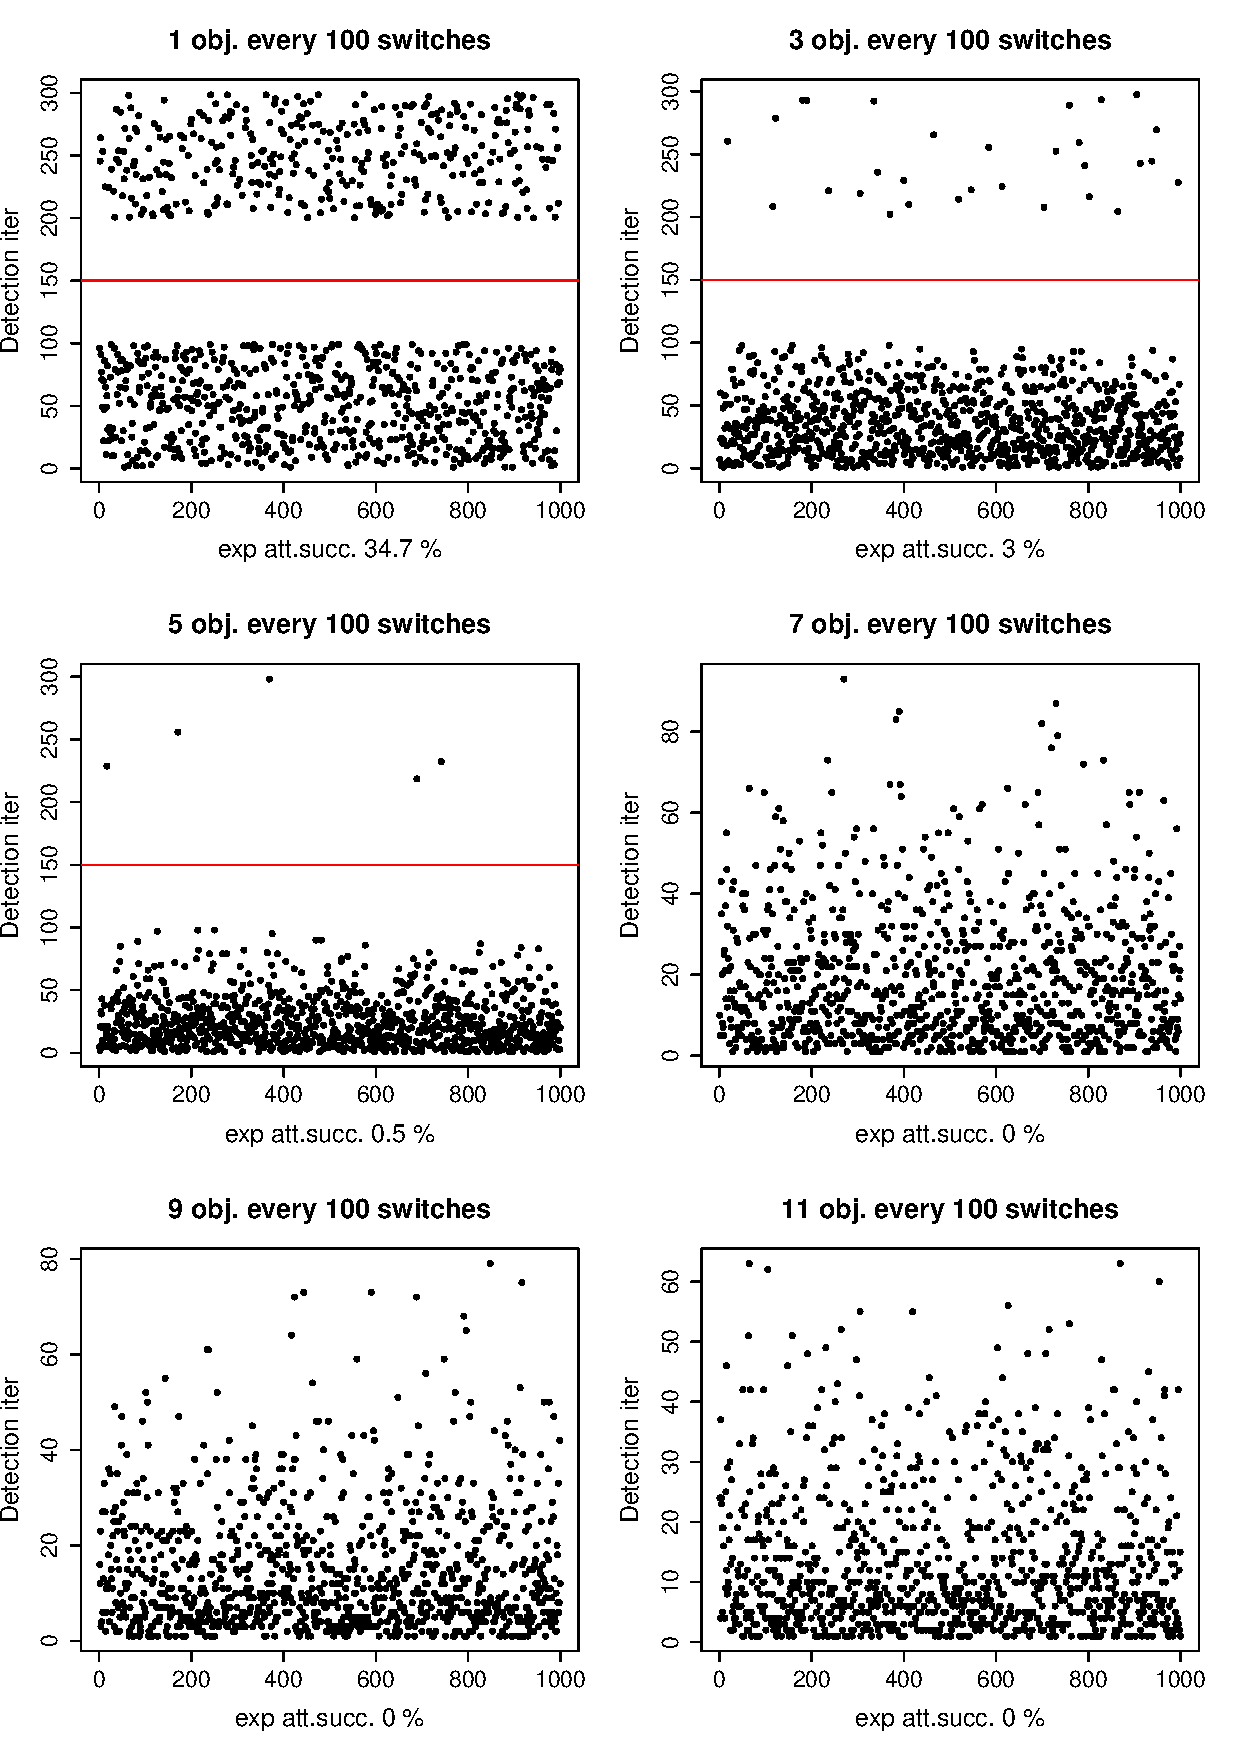
\includegraphics[width=130mm]{images/hr_sim_1000}
\caption{{Monte carlo simulations for the analysis of the probability of attack, compromising from 1 to 11 objects and restoring their original content after 100 task switches}}
\label{monteanalysis}
\end{center}
\end{figure}

The probabilistic nature of selecting a subset of kernel objects to be checked each time, makes our technique susceptible to probabilistic attacks. 
To confirm what we claimed about the effectiveness of the described approach, we provide a Monte Carlo simulation to study the probability of successful attacks in several conditions. 

In Figure \ref{monteanalysis} we plot 1000 runs of our method when 1 to 11 objects are compromised and restored after 100 task switches. If an object stays compromised for a time longer than the one required for 150 task switches, it will certainly be detected ($Pr(detect)=1$) by the hypervisor. Therefore we provide an analysis under condition that is favourable to the attacker.  

In Figure \ref{probts} the probability of successful attacks has been estimated for three cases that consist in restoring the original content of the compromised objects after 75, 90 and 120 task switches respectively.

As expected, this probability is very small ($<< 0.65\%$) when the number of compromised objects is greater than 4 and the number of task switches $TS>100$.



\begin{figure}[htbp]
\begin{center}
\includegraphics[width=70mm, height=85mm]{images/hr_sim_1000_ts}
\caption{{Probability of successful attack compared to restoring rate of 75, 90 and 120 task switches}}
\label{probts}
\end{center}
\end{figure}



A third possible way to compromise the guest kernel would be by corrupting critical kernel objects whose values legitimately change during the kernel's lifetime. Such objects are not invariant and thus cannot  be included in the list of objects that this approach checks since this system is unable to differentiate legitimate from non-legitimate changes. The majority though of existing kernel-mode rootkits modify invariant data structures. Thus our system reduces considerably the rootkit attack surface and prevents most rootkits from performing a successful attack.

Lastly, our method relies on invariance inference engines to provide an accurate list of invariant critical kernel objects. In the worst case scenario, if the designated inference engine does not provide all the invariant critical kernel objects that are interesting targets for attackers (false negatives), this approach will be unable to detect attacks that occur in the non-reported kernel objects.

\clearpage

\section{Related work}\label{hr:related}
Due to the constant development of malicious software and active research in the field, a number of efforts exist on detecting and preventing kernel-mode rootkits. 
In this section we explore related work that attempts to protect a kernel using different technologies such as virtualisation and special-purpose hardware in Section \ref{hardware}, kernel code integrity in Section \ref{integrity} and code profiling in Section \ref{profiling}.


\subsection{Hardware-based countermeasures} \label{hardware}
\paragraph{Copilot}
Copilot \cite{copilot} is a kernel integrity monitor which detects illegal modifications to a host kernel by fetching the physical memory pages where kernel data and code have been stored. The detection strategy of the monitor is based on checking the integrity of kernel data structures with the aid of MD5 hashes. The above detection is performed by a dedicated PCI card, equipped of a coprocessor that fetches kernel pages at regular intervals. Although the measured performance impact is relatively negligible, this mitigation technique is affected by several limitations. Since the detection mechanism is running within the same kernel to protect, the detection will fail when the target kernel is sufficiently modified. As the authors claim in their work, when the kernel itself lies about its integrity, all other system utilities will receive this information and consider it trustworthy. Even in the presence of dedicated hardware, the fact that it is controlled by the target operating system can influence the overall effectiveness of the countermeasure. 
In a testbed similar to the one we propose in our solution, which consists in performing checking of kernel data  every 5 seconds, the overall performance impact has been measured to 3.80\% (WebStone throughput results) compared to the performance of a native system.   
Another shortcoming of Copilot is represented by access limited to main memory: there is no way for Copilot to inspect CPU registers, since it is not possible to pause the CPU's execution of the target system. In our solution, whenever control is returned to the hypervisor, which performs kernel integrity checking, the guest system is paused. A snapshot of the register set of a paused system can be inspected in hypervisor space relatively easily. In our prototype we check the integrity of the Interrupt Descriptor Table Register (IDTR). It goes without saying that the entire register set of the guest machine can be checked with the same mechanism. 
Because Copilot accesses host memory via the PCI bus, there are chances to find kernel data structures in an inconsistent state whenever the monitor performs a DMA access (direct access to physical memory) and a process is modifying them at the same time. Our solution avoids race conditions of this type by invalidating the virtual to physical mapping in the TLB upon returning control to the guest operating system. Specifically, when the hypervisor is repairing (writing) a compromised kernel structure, a process that was using that data before will find an inconsistency. However invalidating the virtual-physical address mapping will force the process to remap the new content stored at the physical address.
The strategy of checking integrity every 30 seconds makes the Copilot monitor susceptible to timing attacks. A rootkit that compromises kernel data and rapidly repairs it will stay unnoticed. Although our mitigation technique is affected by the same problem, we provide a probabilistic analysis that shows the chances of successful timing attacks under several conditions.

\paragraph{Gibraltar}
A system that, similarly to the one described in the previous sections, detects violation of kernel data structures integrity is Gibraltar \cite{6}. Gibraltar executes on a separate machine, called the observer, and monitors the integrity of the kernel running in another machine, physically separated, called the target. Both the observer and the target are connected by the Myrinet PCI intelligent network card. Within such an architecture the observer can remotely access the physical pages of the target kernel. Gibraltar is formed by three main components: the page fetcher, the invariant generator engine and the monitor. The page fetcher, which executes on the observer, fetches the page of a given memory address of the target, where the PCI card has been installed. The PCI device initiates a DMA request for the requested page and send the content back to the observer.
The invariant generator engine, which executes in the observer, generates a list of invariants that conform to several templates, such as membership ($x \in a,b,c$), nonzero ($x \neq 0$), bounds ($x \geq c$, $x \leq c$), etc. The monitor ensures that the list of observed data structures in the memory of the target system satisfy the invariants inferred by the invariant generator engine.
One limitation of Gibraltar is represented by the fact that pages are fetched and monitored asynchronously. Due to the consistent delay between fetching and monitoring, the chances of timing attacks are considerably high.
However, the main limitation is represented by the isolation requirement which is fulfilled by executing the monitor and the target systems within two physically separated machines. The need of special hardware and the overall performance penalty, make Gibraltar not suitable for production systems.  

%FIXME from gibraltar paper  related work TPM can detect certain kinds of rootkits that modify kernel code and critical data structures, but not arbitrary kernel data structures.


\subsection{Kernel code integrity} \label{integrity}

\paragraph{SecVisor}
A countermeasure specifically designed to prevent the execution of unauthorized code is described in \cite{SecVisor}. For the reasons explained in the previous sections, malicious code executing in kernel mode can be extremely dangerous. SecVisor ensures that only approved code can execute in kernel mode. It comes in the form of a tiny hypervisor that operates at VMX root mode, exploiting the virtualisation capabilities of modern hardware architectures like AMD and Intel. By validating kernel code before executing it, SecVisor prevents the execution of injected code, as is the case of kernel rootkits. 
Existing kernel code is also protected in order to prevent any illegal modification from unauthorised parties. In order to achieve the aforementioned goals, SecVisor virtualises the physical memory to set CPU-based memory protections over the kernel, the IO Memory Management Unit (IOMMU) to protect code from DMA writes, and the CPU Memory Management Unit (MMU) in order to check any modification to the MMU from the protected kernel. 
The very limited amount of changes that need to be applied to port an operating system like Linux to execute on SecVisor makes it an attractive solution against rootkits. Unfortunately, the overhead of virtualising memory and shadowing several components of the CPU is very high, compared to other solutions that can achieve the same degree of security.
Another limitation arise from the security evaluation of SecVisor: since control flow integrity is not guaranteed, \emph{return-to-libc} type attacks are still possible. For instance, an attacker can pass control to a kernel function of his choice by overwriting the return address of another function within the same kernel space. Such a  behaviour is considered totally legal by SecVisor.

\paragraph{NICKLE}
A system that prevents the execution of rootkits by detecting the presence of malicious code before its execution is NICKLE \cite{NICKLE}. It comes in the form of a minimal hypervisor which prevents unauthorized kernel code execution. The main advantages of this solutions consists in the fact that it does not require modifications to the guest OS kernel. Therefore commodity OSes can be supported without recompilation or reinstallation. 
To overcome the problem of single memory space for kernel code and user code, NICKLE implements a memory shadowing system that is controlled by the virtual machine monitor and non accessible to the guest. 
The hypervisor maintains a shadow physical memory to store authenticated guest kernel code. Upon the startup of the VM, that is assumed to be in a untampered trusted state, authenticated guest kernel instructions will be copied from the guest's standard memory to the shadow memory controlled by NICKLE. Another specific event that triggers NICKLE's intervention is the loading/unloading of loadable kernel modules. Loading a module is  considered injecting code, that needs to be authenticated and validated before execution. 
At system startup the guest's shadow memory is empty and the system bootstrap code will be verified and copied into the shadow memory. After the kernel has been loaded and decompressed, a cryptographic hash is used to verify its integrity. Then kernel code is copied from standard memory to shadow memory. If the hash values do not match with values computed previously off-line by an administrator or distribution maintainer the code will not be copied to the shadow memory.
The actual protection occurs after validation, when the virtual machine is about to execute a kernel instruction. At this point NICKLE will redirect the instruction fetch to the shadow memory rather than standard memory, after verifying that the current instruction is authenticated. 
Memory accesses to user code, user data and kernel data will proceed without any intervention. 
Kernel rootkit attacks would be detected and prevented since invalidated code would attempt to run in kernel mode.   
A recent attack to bypass countermeasures against code injection attacks, such as the Non-Executable stack countermeasure, is Return Oriented Programming (ROP) \cite{geometry}. In ROP, the attacker, instead of injecting malicious code in the address space of a vulnerable process, crafts his malicious payload by combining fragments of existing code. This method of attacking has been used to create return-oriented rootkits which
re-use fragments of authorized kernel code for malicious purposes \cite{Hund2009}. 
Such rootkits can bypass countermeasures like the ones proposed by \cite{NICKLE, SecVisor}.


\paragraph{Hookscout}
Yin et al. \cite{hookscout} focus on kernel function pointers and protect them from being compromised by rootkits. 
They developed a function pointer protection system called Hookscout. 
The main observation of the authors is that, in many cases, access to source code of the operating system to be protected is not available. Therefore, they provide a binary-centric solution that can generate a hook detection policy without access to the OS kernel source code. 
Their approach is also context-sensitive. This allows detection of kernel hooks even in the presence of polymorphic data structures.
The approach consists of an analysis and a detection phases.
The idea of Hookscout consists in performing dynamic binary analysis of the target system in order to monitor kernel memory objects and keep track of function pointers propagating in kernel space. Since kernel function pointers are the main target of kernel rootkits, the aforementioned analysis can detect how function pointers are created, distributed and used. Moreover all memory objects allocated statically or dynamically are monitored.
The analysis is performed by TEMU, a dynamic binary analysis platform based on QEMU. Therefore the target system needs to be run within an emulator. This is the main cause of the overall performance impact.
During the analysis, the emulated operating system is tested with common test cases, while the monitor engine collects system information such as the state of memory objects and function pointers. Given this information as input to an inference engine, context-sensitive analysis is performed in order to generate the policy for hook detection.
In the detection phase, the detection engine, located within the target system, enforces the policy generated
during the analysis phase and detects hooks in the kernel space at runtime.
It goes without saying that Hookscout's effectiveness can be compromised by a rootkit capable of disabling the protection since the detection system resides within the same target machine.


\paragraph{HookSafe}
Another system that can protect thousands of kernel hooks from being compromised is HookSafe \cite{HookSafe}. Commodity hardware can provide protection with page-level granularity, meaning that protection flags can be set for a page, not for a byte. Since protection of kernel objects needs byte-level granularity, the authors of HookSafe consider the former type of protection not sufficient against rootkits.
HookSafe is a hypervisor-based system that relocates kernel hooks to be protected to a dedicated page and then exploits the regular page-level protection of the MMU to protect that page.
This is doable due to the fact that a kernel hook, once initialized, will be frequently read-accessed and rarely write-accessed. Therefore a relocation of those pointers will not affect the functionality of the overall system.
The concept of shadow memory is used to copy the kernel hooks in a centralised location. Attempts to modify the shadow copy will be trapped by the hypervisor which will verify if the caller has enough permissions to modify the  protected area. Read accesses will be redirected without any intervention to the shadow copy.
A layer between the guest and the hypervisor will handle read and write accesses accordingly. Since the hypervisor is the only component that can write to the memory pages of the protected kernel, control needs to be transferred from the guest to the hypervisor, which will modify on guest's behalf, and then back to the guest kernel.
Kernel rootkits can target areas different from regular memory-based function pointers, such as hardware registers like GDTR, IDTR, SYSENTER and MSR. Being HookSafe a hypervisor-based countermeasure, access to hardware registers can be regulated. Any attempt to write to these registers is intercepted and validated. 
%Related to the hardware register protection is how we secure the GDT and IDT descriptor tables. These two tables contain critical system data structures and their contents must be protected. We protect these two tables using the hardware-based page-level protection.
The main limitation of HookSafe consists in the fact that it does not protect non-control kernel data. Therefore rootkits that target this type of data structures would not be prevented.


\paragraph{SBCFI}
An approach that dynamically monitors operating system kernel integrity is described in \cite{SBCFI}. In this work the authors argue that enforcing control flow integrity can effectively protect against a large class of kernel rootkits. The main observation consists in the fact that, despite the specific behaviour of rootkits (such as injecting code, compromising function pointers, changing the value of specific registers, etc.), the execution flow of a compromised system will differ from the execution flow determined before the attack.
Therefore, control flow integrity can be considered a valuable measure of the integrity of the overall system.
Due to the persistent nature of rootkits, monitoring control flow integrity continuously is not required. Infrequent monitoring can still effectively protect the system and reduce the performance overhead consistently.
SBCFI enforces an approximation of control flow integrity, called state-based control flow integrity. While control flow integrity checks each branch of a precomputed control flow graph in step with the program's execution, SBCFI periodically examines the kernel's state and validate it as a whole.
The target kernel code is first checked for any modification, then all static branches are validated. In a successive phase, all usable function pointers of the heap are verified that they target valid code.
The approximated nature of control flow integrity makes the overhead of SBCFI negligible. Moreover, the control flow integrity monitor can be isolated from the target operating system. 
Both the implementations of SBCFI on top of the Xen hypervisor and the VMware Workstation virtual machine monitor have similar performance impact.




\subsection{Analysis and profiling systems} \label{profiling}
Although not specifically designed to protect against rootkits, malware analysis can reveal important information about the way rootkits can compromise kernel data structures or how private information is stolen, allowing researchers to understand rootkit's behaviour and design effective countermeasures against them. 
Most state-of-the-art analysis approaches share the same execution space of the malware that is being analysed. This can reduce the value and effectiveness of the analysis because some malware can detect the analysis platform and behave differently than in the real target system. 
The isolation capability of virtualisation technology and the ability to save and restore the state of a guest operating system are offering new tools to shed light on the complex techniques of malware development. 
General purpose hypervisors are usually not suitable for the purpose of analysing malware because they provide access to an emulated version of the hardware making the entire virtualisation platform visible to complex malicious software. 
Recent malware like Storm and Conficker are known to detect they are running inside a virtual machine and behave differently \cite{conficker, ecards}


\paragraph{MAVMM}
MAVMM \cite{MAVMM} is a virtual machine monitor specifically designed for malware analysis. It can extract useful information for a complete profile of the investigated malware such as memory pages, system calls and accesses to disks and network devices. Contrarily to other hypervisors, MAVMM lets most hardware access requests go through without interception. This feature makes the entire platform invisible to the malware while still controlling accesses to the aformentioned areas of the system. The analysis platform only intercepts guest execution at a few places, in order to protect its own integrity and log the guests' behaviours for further analysis. Hardware supported Nested Page Tables (NPT) are used to protect its memory from being compromised by the guest, while an IOMMU unit is used to prevent any tamper by external hardware devices via DMA.
The execution trace of a guest program is recorded by single stepping its execution at each instruction. This is implemented by virtualising the TF flag that will raise a debugger exception, which will in turn be intercepted by MAVMM. 
A log of executed system calls can give a good picture of what the malware under investigation is trying to do. MAVMM can record all system calls that a guest system invokes during its lifetime. Selective analysis of specific processes in the guest is also possible by notifying MAVMM each time a process switch occurs in the guest.
An issue to deal with consists in choosing the safest place to store collected information for further analysis. Using the same disk device would expose collected data to be compromised by the analysed malware. Therefore, an USB flash drive or a separate disk unit controlled by different device drivers is an approach preferred by the authors.



\paragraph{Hookmap}
Wang et al. \cite{hookmap} is an analysis tool against persistent rootkits based on the observation that rootkits try to hide their presence within the target kernel and they usually install kernel hooks on the corresponding kernel-side execution path invoked by the target program. Therefore given a security program, the authors argue that it is sufficient to analyse its kernel-side execution path to detect and investigate the rootkit behaviour. Linux utility programs like \emph{ls}, \emph{ps} and \emph{netstat} have been analysed and their relative kernel hooks identified. HookMap found that there are 35 kernel hooks mapped to the \emph{ls} utility, 85 kernel hooks for \emph{ps} and so forth. As a result it is a systematic approach to uncover kernel hooks that can be potentially hijacked. By recording possible control-flow transfer instructions in the kernel-side execution paths HookMap is able to derive all related kernel hooks. For isolation purposes HookMap is based on QEMU and the target operating system is running within a virtual machine environment. 


\paragraph{HookFinder}
An approach that does not rely on any prior knowledge of hooking mechanisms is HookFinder \cite{hookfinder}. Therefore it represents a suitable tool to identify novel hooking mechanisms. To overcome the limitation of static analysis, that can be easily circumvented by malicious programs equipped with code obfuscation techniques, HookFinder relies on dynamic analysis. This means that malware programs are analysed while being executed within a controlled environment. A whole-system emulator is used for the purpose. All the information collected by the three main components of HookFinder, namely the impact engine, the hook detector and the semantics extractor, is used to derive how the rootkit implants the hook and how the hook is activated by the operating system. When the malware starts executing, the initial impacts, that is data written directly by the malicious code (and by external components, on behalf of malicious code) are added to a list to be monitored. Then HookFinder keeps track of the impacts propagating through the whole system. For instance, if it is observed that the instruction pointer is loaded with a monitored impact, and the execution jumps immediately into the malicious code, then a hook has been identified.
Once a hook has been identified, HookFinder records into a trace the details about the propagated impacts in the system. By combining the information of the trace and operating system level semantics, HookFinder finally provides an intuitive graphical representation that can be used by malware analysts for a better understanding of the hooking mechanism under investigation.



\paragraph{PoKer}
Another virtualisation-based rootkit profiler is described in \cite{PoKer}. PoKer can log the rootkit hooking behaviour, it can monitor targeted kernel objects, extract kernel rootkit code and infer the potential impact on user-level programs. Poker is deployed in systems that can tolerate non negligible performance impact such as honeypots, for which correctly profiling a rootkit has a higher priority than profiling it faster. The overall system with PoKer enabled executes 3.8 times slower then the equivalent system without PoKer.
The profiler will be enabled after the first malicious instruction has been executed. The techniques described by NICKLE and SecVisor are considered by PoKer to ensure that all actions are logged after this specific event.
At this point, PoKer switches to a rootkit profiling mode, by activating a separate virtual machine, and starts to determine the static and dynamic objects that are being targeted by the rootkit. In order to accurately profile compromised objects, PoKer needs to access the source code of the operating system kernel or debugging symbols and type information of a compiled kernel binary. Gathered information is stored outside the target virtual machine, to prevent any tamper with the rootkit under investigation.
Interpreting the traces and resolving read and write target addresses is considered a challenging task, due to the difficulty of identifying the corresponding kernel object, given an arbitrary memory address.
Since virtualisation technology does not support such a reverse lookup, an address-to-dynamic object table map is used to translate memory addresses into kernel objects. An initial map of static objects, combined to the rootkit's reads is a sufficient information to build the aforementioned map on the fly.



The countermeasure described in the previous sections can be integrated with the systems described above in order to perform integrity checking and detect illegal changes to those kernel objects collected by the aforementioned analysis tools.


\section{Summary}\label{hr:conclusion}
In this chapter we showed the effectiveness of the isolation between a hypervisor and a guest operating system and demonstrated how to build a non-bypassable invariance-enforcing framework that takes advantage of this feature.
We realised our idea by designing and implementing a lightweight countermeasure that mitigates the problem of kernel-mode rootkits in common operating system kernels.

Upon detection of a change of an invariant kernel object, our countermeasure alerts the administrator of the guest operating system and proceeds to repair the kernel by restoring the data structure to its original values. Due to this change, the rootkit's injected code is usually no longer reachable by any statements in the kernel and thus can no longer affect the running kernel's operations. 

The performance impact that usually affects virtualisation technology has been consistently reduced by relaxing the problem of protecting a high number of kernel data structures, without limiting the security degree of the countermeasure. A probabilistic analysis has been provided in order to assess the impact of the aforementioned relaxation, in terms of security. 
Moreover, our prototype has been evaluated on synthetic and real rootkits and it has been showed that it can detect control-flow changes with negligible performance and memory overhead, making it a viable countermeasure for protecting operating systems in virtualised environments.

The limit of 15000 critical kernel objects holds only in the prototype. However we consider it an acceptable amount that can protect a high number of kernel data structures and function pointers. 
Although the attack surface results dramatically reduced, attacks to variant data structures are still possible. However, a different strategy and system's design must be investigated in order to overtake such a limitation. We believe that research in that direction is needed as more virtualisation-based systems are making their appearance on the scene. 
